% Options for packages loaded elsewhere
\PassOptionsToPackage{unicode}{hyperref}
\PassOptionsToPackage{hyphens}{url}
\PassOptionsToPackage{dvipsnames,svgnames,x11names}{xcolor}
%
\documentclass[
  letterpaper,
  DIV=11,
  numbers=noendperiod]{scrartcl}

\usepackage{amsmath,amssymb}
\usepackage{lmodern}
\usepackage{iftex}
\ifPDFTeX
  \usepackage[T1]{fontenc}
  \usepackage[utf8]{inputenc}
  \usepackage{textcomp} % provide euro and other symbols
\else % if luatex or xetex
  \usepackage{unicode-math}
  \defaultfontfeatures{Scale=MatchLowercase}
  \defaultfontfeatures[\rmfamily]{Ligatures=TeX,Scale=1}
\fi
% Use upquote if available, for straight quotes in verbatim environments
\IfFileExists{upquote.sty}{\usepackage{upquote}}{}
\IfFileExists{microtype.sty}{% use microtype if available
  \usepackage[]{microtype}
  \UseMicrotypeSet[protrusion]{basicmath} % disable protrusion for tt fonts
}{}
\makeatletter
\@ifundefined{KOMAClassName}{% if non-KOMA class
  \IfFileExists{parskip.sty}{%
    \usepackage{parskip}
  }{% else
    \setlength{\parindent}{0pt}
    \setlength{\parskip}{6pt plus 2pt minus 1pt}}
}{% if KOMA class
  \KOMAoptions{parskip=half}}
\makeatother
\usepackage{xcolor}
\setlength{\emergencystretch}{3em} % prevent overfull lines
\setcounter{secnumdepth}{-\maxdimen} % remove section numbering
% Make \paragraph and \subparagraph free-standing
\ifx\paragraph\undefined\else
  \let\oldparagraph\paragraph
  \renewcommand{\paragraph}[1]{\oldparagraph{#1}\mbox{}}
\fi
\ifx\subparagraph\undefined\else
  \let\oldsubparagraph\subparagraph
  \renewcommand{\subparagraph}[1]{\oldsubparagraph{#1}\mbox{}}
\fi

\usepackage{color}
\usepackage{fancyvrb}
\newcommand{\VerbBar}{|}
\newcommand{\VERB}{\Verb[commandchars=\\\{\}]}
\DefineVerbatimEnvironment{Highlighting}{Verbatim}{commandchars=\\\{\}}
% Add ',fontsize=\small' for more characters per line
\usepackage{framed}
\definecolor{shadecolor}{RGB}{241,243,245}
\newenvironment{Shaded}{\begin{snugshade}}{\end{snugshade}}
\newcommand{\AlertTok}[1]{\textcolor[rgb]{0.68,0.00,0.00}{#1}}
\newcommand{\AnnotationTok}[1]{\textcolor[rgb]{0.37,0.37,0.37}{#1}}
\newcommand{\AttributeTok}[1]{\textcolor[rgb]{0.40,0.45,0.13}{#1}}
\newcommand{\BaseNTok}[1]{\textcolor[rgb]{0.68,0.00,0.00}{#1}}
\newcommand{\BuiltInTok}[1]{\textcolor[rgb]{0.00,0.23,0.31}{#1}}
\newcommand{\CharTok}[1]{\textcolor[rgb]{0.13,0.47,0.30}{#1}}
\newcommand{\CommentTok}[1]{\textcolor[rgb]{0.37,0.37,0.37}{#1}}
\newcommand{\CommentVarTok}[1]{\textcolor[rgb]{0.37,0.37,0.37}{\textit{#1}}}
\newcommand{\ConstantTok}[1]{\textcolor[rgb]{0.56,0.35,0.01}{#1}}
\newcommand{\ControlFlowTok}[1]{\textcolor[rgb]{0.00,0.23,0.31}{#1}}
\newcommand{\DataTypeTok}[1]{\textcolor[rgb]{0.68,0.00,0.00}{#1}}
\newcommand{\DecValTok}[1]{\textcolor[rgb]{0.68,0.00,0.00}{#1}}
\newcommand{\DocumentationTok}[1]{\textcolor[rgb]{0.37,0.37,0.37}{\textit{#1}}}
\newcommand{\ErrorTok}[1]{\textcolor[rgb]{0.68,0.00,0.00}{#1}}
\newcommand{\ExtensionTok}[1]{\textcolor[rgb]{0.00,0.23,0.31}{#1}}
\newcommand{\FloatTok}[1]{\textcolor[rgb]{0.68,0.00,0.00}{#1}}
\newcommand{\FunctionTok}[1]{\textcolor[rgb]{0.28,0.35,0.67}{#1}}
\newcommand{\ImportTok}[1]{\textcolor[rgb]{0.00,0.46,0.62}{#1}}
\newcommand{\InformationTok}[1]{\textcolor[rgb]{0.37,0.37,0.37}{#1}}
\newcommand{\KeywordTok}[1]{\textcolor[rgb]{0.00,0.23,0.31}{#1}}
\newcommand{\NormalTok}[1]{\textcolor[rgb]{0.00,0.23,0.31}{#1}}
\newcommand{\OperatorTok}[1]{\textcolor[rgb]{0.37,0.37,0.37}{#1}}
\newcommand{\OtherTok}[1]{\textcolor[rgb]{0.00,0.23,0.31}{#1}}
\newcommand{\PreprocessorTok}[1]{\textcolor[rgb]{0.68,0.00,0.00}{#1}}
\newcommand{\RegionMarkerTok}[1]{\textcolor[rgb]{0.00,0.23,0.31}{#1}}
\newcommand{\SpecialCharTok}[1]{\textcolor[rgb]{0.37,0.37,0.37}{#1}}
\newcommand{\SpecialStringTok}[1]{\textcolor[rgb]{0.13,0.47,0.30}{#1}}
\newcommand{\StringTok}[1]{\textcolor[rgb]{0.13,0.47,0.30}{#1}}
\newcommand{\VariableTok}[1]{\textcolor[rgb]{0.07,0.07,0.07}{#1}}
\newcommand{\VerbatimStringTok}[1]{\textcolor[rgb]{0.13,0.47,0.30}{#1}}
\newcommand{\WarningTok}[1]{\textcolor[rgb]{0.37,0.37,0.37}{\textit{#1}}}

\providecommand{\tightlist}{%
  \setlength{\itemsep}{0pt}\setlength{\parskip}{0pt}}\usepackage{longtable,booktabs,array}
\usepackage{calc} % for calculating minipage widths
% Correct order of tables after \paragraph or \subparagraph
\usepackage{etoolbox}
\makeatletter
\patchcmd\longtable{\par}{\if@noskipsec\mbox{}\fi\par}{}{}
\makeatother
% Allow footnotes in longtable head/foot
\IfFileExists{footnotehyper.sty}{\usepackage{footnotehyper}}{\usepackage{footnote}}
\makesavenoteenv{longtable}
\usepackage{graphicx}
\makeatletter
\def\maxwidth{\ifdim\Gin@nat@width>\linewidth\linewidth\else\Gin@nat@width\fi}
\def\maxheight{\ifdim\Gin@nat@height>\textheight\textheight\else\Gin@nat@height\fi}
\makeatother
% Scale images if necessary, so that they will not overflow the page
% margins by default, and it is still possible to overwrite the defaults
% using explicit options in \includegraphics[width, height, ...]{}
\setkeys{Gin}{width=\maxwidth,height=\maxheight,keepaspectratio}
% Set default figure placement to htbp
\makeatletter
\def\fps@figure{htbp}
\makeatother

\KOMAoption{captions}{tableheading}
\makeatletter
\makeatother
\makeatletter
\makeatother
\makeatletter
\@ifpackageloaded{caption}{}{\usepackage{caption}}
\AtBeginDocument{%
\ifdefined\contentsname
  \renewcommand*\contentsname{Table of contents}
\else
  \newcommand\contentsname{Table of contents}
\fi
\ifdefined\listfigurename
  \renewcommand*\listfigurename{List of Figures}
\else
  \newcommand\listfigurename{List of Figures}
\fi
\ifdefined\listtablename
  \renewcommand*\listtablename{List of Tables}
\else
  \newcommand\listtablename{List of Tables}
\fi
\ifdefined\figurename
  \renewcommand*\figurename{Figure}
\else
  \newcommand\figurename{Figure}
\fi
\ifdefined\tablename
  \renewcommand*\tablename{Table}
\else
  \newcommand\tablename{Table}
\fi
}
\@ifpackageloaded{float}{}{\usepackage{float}}
\floatstyle{ruled}
\@ifundefined{c@chapter}{\newfloat{codelisting}{h}{lop}}{\newfloat{codelisting}{h}{lop}[chapter]}
\floatname{codelisting}{Listing}
\newcommand*\listoflistings{\listof{codelisting}{List of Listings}}
\makeatother
\makeatletter
\@ifpackageloaded{caption}{}{\usepackage{caption}}
\@ifpackageloaded{subcaption}{}{\usepackage{subcaption}}
\makeatother
\makeatletter
\@ifpackageloaded{tcolorbox}{}{\usepackage[many]{tcolorbox}}
\makeatother
\makeatletter
\@ifundefined{shadecolor}{\definecolor{shadecolor}{rgb}{.97, .97, .97}}
\makeatother
\makeatletter
\makeatother
\ifLuaTeX
  \usepackage{selnolig}  % disable illegal ligatures
\fi
\IfFileExists{bookmark.sty}{\usepackage{bookmark}}{\usepackage{hyperref}}
\IfFileExists{xurl.sty}{\usepackage{xurl}}{} % add URL line breaks if available
\urlstyle{same} % disable monospaced font for URLs
\hypersetup{
  pdftitle={Case-Control Point Data Homework (First- and Second-Order Properties)},
  colorlinks=true,
  linkcolor={blue},
  filecolor={Maroon},
  citecolor={Blue},
  urlcolor={Blue},
  pdfcreator={LaTeX via pandoc}}

\title{Case-Control Point Data Homework (First- and Second-Order
Properties)}
\author{}
\date{}

\begin{document}
\maketitle
\ifdefined\Shaded\renewenvironment{Shaded}{\begin{tcolorbox}[boxrule=0pt, borderline west={3pt}{0pt}{shadecolor}, enhanced, breakable, interior hidden, frame hidden, sharp corners]}{\end{tcolorbox}}\fi

Instructions: Answer the following questions and write your answers in a
word processor. Mathematical symbols should be written using the
equation editor. Appropriate graphics should be included. The document
may also be created in LaTeX, though this is NOT encouraged.

\hypertarget{problem-1}{%
\section{Problem 1}\label{problem-1}}

The \texttt{urkiola} data set in the \textbf{spatstat package} contains
locations of birch (Betula celtiberica) and oak (Quercus robur) trees in
a secondary wood in Urkiola Natural Park (Basque country, northern
Spain). They are part of a more extensive dataset collected and analysed
by Laskurain (2008). The coordinates of the trees are given in meters.
Let the ``oak'' trees be the cases and ``birch'' trees be the controls.

\hypertarget{a.}{%
\subsection{a.}\label{a.}}

Create a plot of the of the point pattern that distinguishes between the
two types of trees. Do you notice any evidence of clusters? Explain.

\begin{Shaded}
\begin{Highlighting}[]
\FunctionTok{library}\NormalTok{(spatstat)}
\end{Highlighting}
\end{Shaded}

\begin{verbatim}
Loading required package: spatstat.data
\end{verbatim}

\begin{verbatim}
Loading required package: spatstat.geom
\end{verbatim}

\begin{verbatim}
spatstat.geom 3.2-5
\end{verbatim}

\begin{verbatim}
Loading required package: spatstat.random
\end{verbatim}

\begin{verbatim}
spatstat.random 3.1-6
\end{verbatim}

\begin{verbatim}
Loading required package: spatstat.explore
\end{verbatim}

\begin{verbatim}
Loading required package: nlme
\end{verbatim}

\begin{verbatim}
spatstat.explore 3.2-3
\end{verbatim}

\begin{verbatim}
Loading required package: spatstat.model
\end{verbatim}

\begin{verbatim}
Loading required package: rpart
\end{verbatim}

\begin{verbatim}
spatstat.model 3.2-6
\end{verbatim}

\begin{verbatim}
Loading required package: spatstat.linnet
\end{verbatim}

\begin{verbatim}
spatstat.linnet 3.1-1
\end{verbatim}

\begin{verbatim}

spatstat 3.0-6 
For an introduction to spatstat, type 'beginner' 
\end{verbatim}

\begin{Shaded}
\begin{Highlighting}[]
\FunctionTok{library}\NormalTok{(ggplot2)}

\NormalTok{urk }\OtherTok{\textless{}{-}}\NormalTok{ spatstat.data}\SpecialCharTok{::}\NormalTok{urkiola}
\FunctionTok{plot}\NormalTok{(urk,}\AttributeTok{cols=}\FunctionTok{c}\NormalTok{(}\StringTok{\textquotesingle{}blue\textquotesingle{}}\NormalTok{,}\StringTok{\textquotesingle{}green\textquotesingle{}}\NormalTok{),}\AttributeTok{main =} \StringTok{\textquotesingle{}Urkiola Birch and Oak Locations\textquotesingle{}}\NormalTok{)}
\end{Highlighting}
\end{Shaded}

\begin{figure}[H]

{\centering 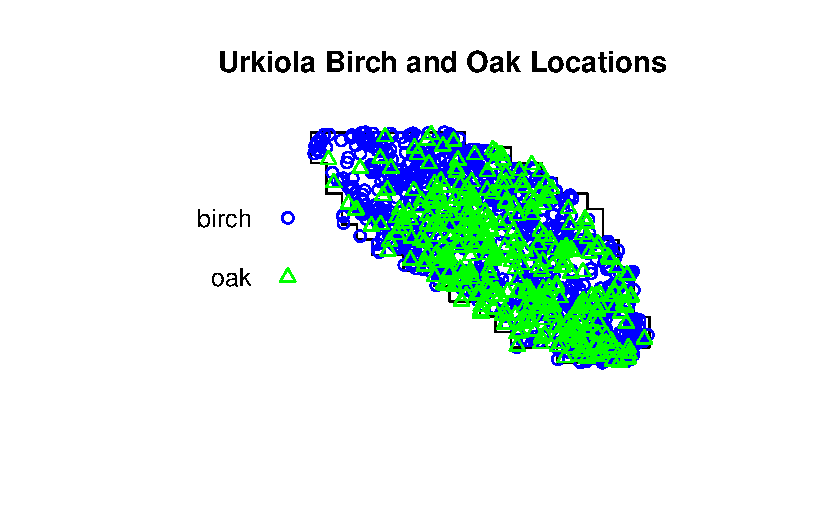
\includegraphics{cc-r-kd-hw_files/figure-pdf/unnamed-chunk-1-1.pdf}

}

\end{figure}

\begin{quote}
From the above plot we can see areas where more birch trees appear to be
prominent relative to the oak trees but it is hard to say if the oak
trees are clustering in a different manner than the birch locations. It
does appear that there are fewer oak trees found in the upper left
region while the oak trees do appear more plentiful in the inner
regions.
\end{quote}

\hypertarget{b.}{%
\subsection{b.}\label{b.}}

Create contour plots of the spatial density function for the oak and
birch trees. Use a bandwidth of 14.5 for the oak trees and 15 for the
birch trees. Do any differences jump out to you?

\begin{Shaded}
\begin{Highlighting}[]
\FunctionTok{library}\NormalTok{(smacpod)}

\NormalTok{oak }\OtherTok{\textless{}{-}} \FunctionTok{which}\NormalTok{(urk}\SpecialCharTok{$}\NormalTok{marks }\SpecialCharTok{==} \StringTok{\textquotesingle{}oak\textquotesingle{}}\NormalTok{)}
\NormalTok{birch }\OtherTok{\textless{}{-}} \FunctionTok{which}\NormalTok{(urk}\SpecialCharTok{$}\NormalTok{marks }\SpecialCharTok{==} \StringTok{\textquotesingle{}birch\textquotesingle{}}\NormalTok{)}



\NormalTok{oak\_sp }\OtherTok{\textless{}{-}} \FunctionTok{spdensity}\NormalTok{(urk[oak],}\AttributeTok{sigma=}\FloatTok{14.5}\NormalTok{)}
\NormalTok{birch\_sp }\OtherTok{\textless{}{-}} \FunctionTok{spdensity}\NormalTok{(urk[birch],}\AttributeTok{sigma=}\DecValTok{15}\NormalTok{)}



\CommentTok{\# contour plot of oak with title}
\FunctionTok{contour}\NormalTok{(oak\_sp, }\AttributeTok{nlevels =} \DecValTok{15}\NormalTok{, }\AttributeTok{main =} \StringTok{""}\NormalTok{)}
\FunctionTok{title}\NormalTok{(}\StringTok{"Oak, bandwidth = 14.5"}\NormalTok{)}
\end{Highlighting}
\end{Shaded}

\begin{figure}[H]

{\centering 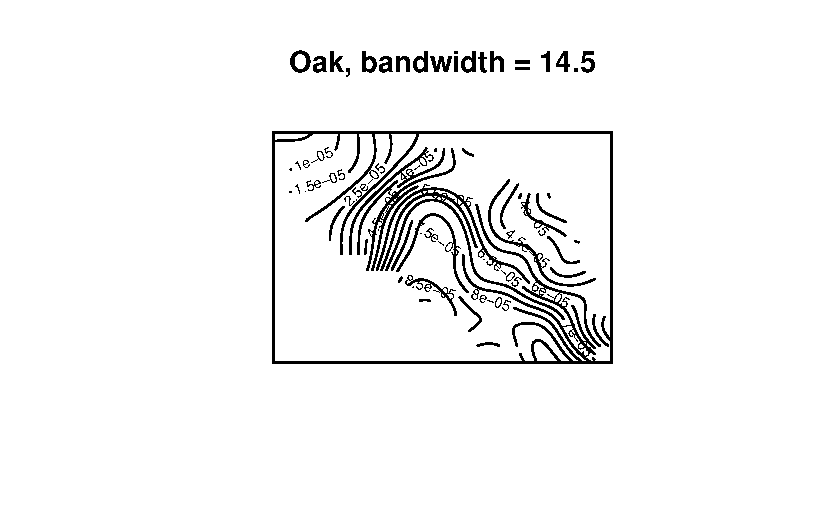
\includegraphics{cc-r-kd-hw_files/figure-pdf/unnamed-chunk-2-1.pdf}

}

\end{figure}

\begin{Shaded}
\begin{Highlighting}[]
\CommentTok{\# contour plot of birch, with title}
\FunctionTok{contour}\NormalTok{(birch\_sp, }\AttributeTok{nlevels =} \DecValTok{15}\NormalTok{, }\AttributeTok{main =} \StringTok{""}\NormalTok{)}
\FunctionTok{title}\NormalTok{(}\StringTok{"Birch, bandwidth = 15"}\NormalTok{)}
\end{Highlighting}
\end{Shaded}

\begin{figure}[H]

{\centering 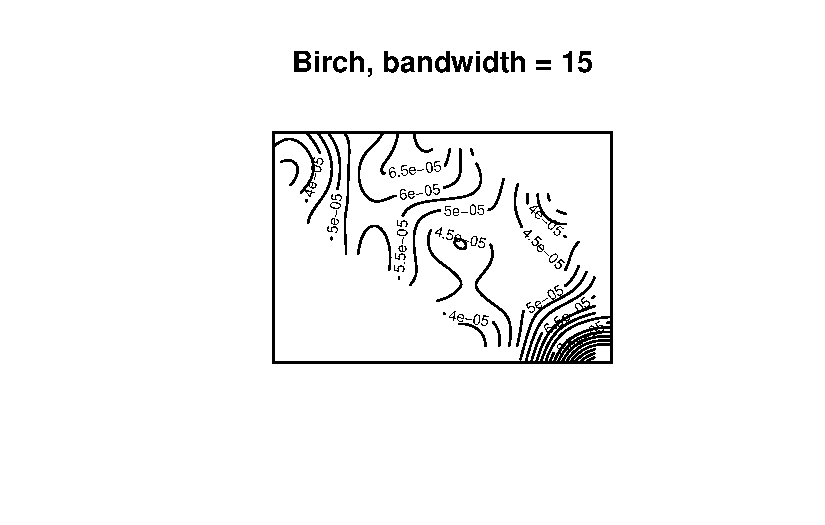
\includegraphics{cc-r-kd-hw_files/figure-pdf/unnamed-chunk-2-2.pdf}

}

\end{figure}

\begin{quote}
The contour plots show some differences between the oak and birch
intensities. It appears that in both plots the intensities are flatter
in some areas relative to other areas but these locations do not match
between the oak and birch plots. This implies that the relative
intensities between birch and oak tree locations are different.
\end{quote}

\hypertarget{c.}{%
\subsection{c.}\label{c.}}

Estimate the log ratio of the spatial density of the oak trees relative
to the birch trees (\(r(s)\)) using a bandwidth of 16. Create a contour
plot of the log ratio. Which areas are most inconsistent with the belief
that the spatial densities for the two types of trees are the same?

\begin{Shaded}
\begin{Highlighting}[]
\CommentTok{\# log ratio of spatial densities}
\NormalTok{r\_oak }\OtherTok{=} \FunctionTok{logrr}\NormalTok{(urk, }\AttributeTok{case =} \StringTok{"oak"}\NormalTok{, }\AttributeTok{sigma =} \DecValTok{16}\NormalTok{)}
\end{Highlighting}
\end{Shaded}

\begin{verbatim}
oak has been selected as the case group
\end{verbatim}

\begin{Shaded}
\begin{Highlighting}[]
\CommentTok{\# contour plot of r\_oak}
\FunctionTok{contour}\NormalTok{(r\_oak, }\AttributeTok{lty =} \FunctionTok{c}\NormalTok{(}\DecValTok{1}\NormalTok{, }\DecValTok{1}\NormalTok{, }\DecValTok{1}\NormalTok{, }\DecValTok{1}\NormalTok{, }\DecValTok{2}\NormalTok{, }\DecValTok{1}\NormalTok{),}
        \AttributeTok{lwd =} \FunctionTok{c}\NormalTok{(}\DecValTok{1}\NormalTok{, }\DecValTok{1}\NormalTok{, }\DecValTok{1}\NormalTok{, }\DecValTok{1}\NormalTok{, }\DecValTok{1}\NormalTok{, }\DecValTok{2}\NormalTok{), }\AttributeTok{main =} \StringTok{""}\NormalTok{)}
\FunctionTok{title}\NormalTok{(}\StringTok{"Gaussian kernel, Bandwidth = 16"}\NormalTok{)}
\end{Highlighting}
\end{Shaded}

\begin{figure}[H]

{\centering 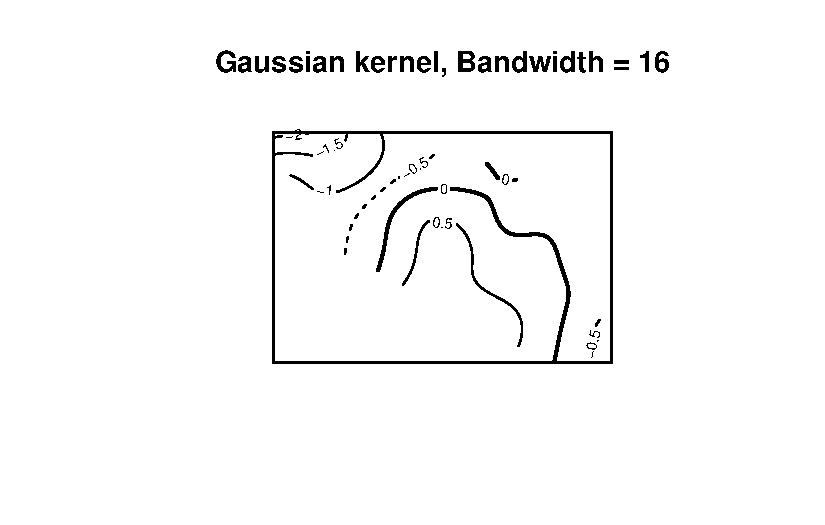
\includegraphics{cc-r-kd-hw_files/figure-pdf/unnamed-chunk-3-1.pdf}

}

\end{figure}

\begin{quote}
The region in the top left of the plot are inconsistent with the belief
that the spatial densities are the same for both tree types.
\end{quote}

\hypertarget{d.}{%
\subsection{d.}\label{d.}}

Construct pointwise 95\% tolerance envelopes for \(r(s)\) using 499 data
sets simulated under the random labeling hypothesis. Plot the regions
above and below the tolerance envelopes in different colors. Overlay the
contour plot of \(\tilde{r}(s)\). What can you conclude?

\begin{Shaded}
\begin{Highlighting}[]
\CommentTok{\# construct 95\% tolerance envelopes for log relative risk}
\NormalTok{lrr\_oak }\OtherTok{=} \FunctionTok{logrr}\NormalTok{(urk, }\AttributeTok{sigma =} \DecValTok{16}\NormalTok{, }\AttributeTok{case =} \StringTok{\textquotesingle{}oak\textquotesingle{}}\NormalTok{, }\AttributeTok{nsim =} \DecValTok{499}\NormalTok{,}
                \AttributeTok{level =} \FloatTok{0.95}\NormalTok{)}
\end{Highlighting}
\end{Shaded}

\begin{verbatim}
oak has been selected as the case group
\end{verbatim}

\begin{Shaded}
\begin{Highlighting}[]
\FunctionTok{plot}\NormalTok{(lrr\_oak)}
\end{Highlighting}
\end{Shaded}

\begin{figure}[H]

{\centering 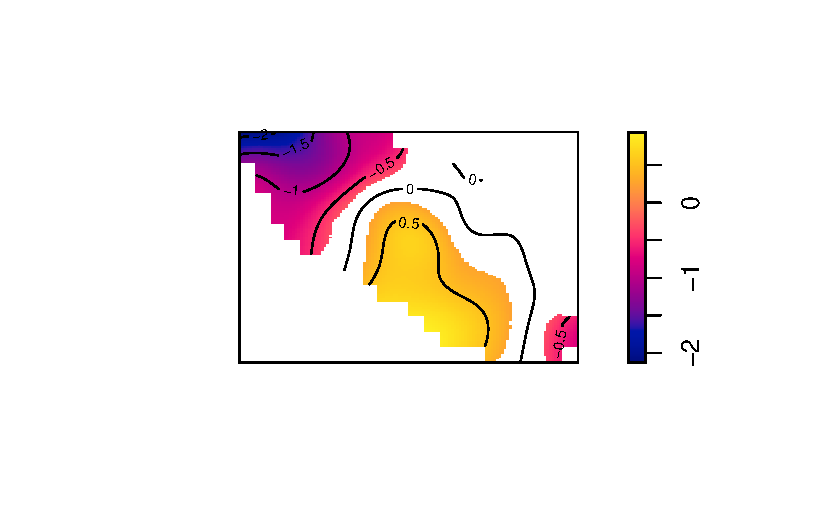
\includegraphics{cc-r-kd-hw_files/figure-pdf/unnamed-chunk-4-1.pdf}

}

\end{figure}

\begin{quote}
From the overlaid contour plot, we can see evidence of birch tree
clustering relative to oak trees in the upper left region and far bottom
right region. Alternatively, in the center we actually see evidence of
the oak trees clustering relative to the birch tree locations.
\end{quote}

\hypertarget{e.}{%
\subsection{e.}\label{e.}}

Perform a global test of clustering using \(\tilde{r}(s)\). Is there
convincing evidence of clustering of one group relative to the other for
at least one location in the study area?.

\begin{Shaded}
\begin{Highlighting}[]
\FunctionTok{logrr.test}\NormalTok{(lrr\_oak)}
\end{Highlighting}
\end{Shaded}

\begin{verbatim}

Kelsall and Diggle (1995) test for log relative risk

r(s) = ln[f(s)/g(s)]
f(s) = spatial density of cases at location s
g(s) = spatial density of controls at location s
case label:  oak 
control label:  birch 

null hypothesis: r(s) = 0 for all s in study area
alternative hypothesis: r(s) != 0 for at least one s in study area
test statistic: 7839.597 
p-value: 0.002 
nsim: 499 
simulation procedure: random labeling
\end{verbatim}

\begin{quote}
Yes, we can reject the null hypothesis that r(s) = 0 for all s at the
alpha=0.05 level. This implies that there is evidence of clustering of
the cases relative to the controls.
\end{quote}

\hypertarget{f.}{%
\subsection{f.}\label{f.}}

Construct a plot for the difference in K functions between the oak trees
and the birch trees. Also include min/max envelopes for this difference
using 499 simulated data sets under the random labeling hypothesis. Also
construct 95\% pointwise tolerance envelopes. Also include the mean
difference from the simulations. Provide a legend labeling these things.
Are there any spatial scales for which the oak trees are more clustered
than the birch trees in comparison to what we expect under the random
labeling hypothesis (or vice versa)? If so, what scales?

\begin{Shaded}
\begin{Highlighting}[]
\DocumentationTok{\#\#\# difference in K functions}
\CommentTok{\# estimate K function for birch and oak,}
\CommentTok{\# take their difference}
\NormalTok{kd }\OtherTok{=} \FunctionTok{kdest}\NormalTok{(urk, }\AttributeTok{case =} \StringTok{\textquotesingle{}oak\textquotesingle{}}\NormalTok{)}
\end{Highlighting}
\end{Shaded}

\begin{verbatim}
oak has been selected as the case group
\end{verbatim}

\begin{Shaded}
\begin{Highlighting}[]
\CommentTok{\# plot estimated and theoretical KD (under RLH)}
\FunctionTok{plot}\NormalTok{(kd, }\FunctionTok{cbind}\NormalTok{(iso, theo) }\SpecialCharTok{\textasciitilde{}}\NormalTok{ r, }\AttributeTok{legend =} \ConstantTok{FALSE}\NormalTok{, }\AttributeTok{main =} \StringTok{""}\NormalTok{)}
\end{Highlighting}
\end{Shaded}

\begin{figure}[H]

{\centering 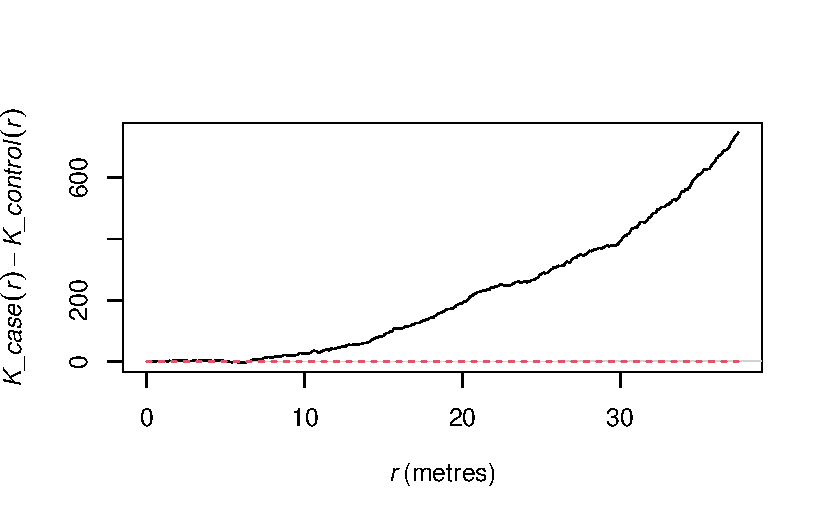
\includegraphics{cc-r-kd-hw_files/figure-pdf/unnamed-chunk-6-1.pdf}

}

\end{figure}

\begin{Shaded}
\begin{Highlighting}[]
\CommentTok{\# construct envelopes using 499 randomly labeled data sets}

\NormalTok{kdenv }\OtherTok{=} \FunctionTok{kdest}\NormalTok{(urk, }\AttributeTok{case =} \StringTok{"oak"}\NormalTok{, }\AttributeTok{nsim =} \DecValTok{499}\NormalTok{,}
              \AttributeTok{level =} \FloatTok{0.95}\NormalTok{)}
\end{Highlighting}
\end{Shaded}

\begin{verbatim}
oak has been selected as the case group
\end{verbatim}

\begin{verbatim}
Generating 499 simulations by evaluating expression  ...
1, 2, 3, .5 [4:44 remaining] ...
.10 [4:46 remaining] ....15 [4:38 remaining] ....20 [4:32 remaining] ..
..25 [4:28 remaining] ....30 [4:24 remaining] ....35 [4:21 remaining] .
...40 [4:18 remaining] ....45 [4:15 remaining] ....50
 [4:12 remaining] ....55 [4:09 remaining] ....60 [4:05 remaining] ....
65 [4:03 remaining] ....70 [3:59 remaining] ....75 [3:57 remaining] ...
.80 [3:54 remaining] ....85 [3:51 remaining] ....90 [3:48 remaining] ..
..95 [3:45 remaining] ....100 [3:42 remaining] ....105 [3:39 remaining] .
...110 [3:36 remaining] ....115 [3:33 remaining] ....120
 [3:31 remaining] ....125 [3:28 remaining] ....130 [3:25 remaining] ....
135 [3:22 remaining] ....140 [3:19 remaining] ....145 [3:17 remaining] ...
.150 [3:14 remaining] ....155 [3:11 remaining] ....160 [3:08 remaining] ..
..165 [3:05 remaining] ....170 [3:03 remaining] ....175 [3:00 remaining] .
...180 [2:57 remaining] ....185 [2:55 remaining] ....190
 [2:52 remaining] ....195 [2:49 remaining] ....200 [2:46 remaining] ....
205 [2:43 remaining] ....210 [2:41 remaining] ....215 [2:38 remaining] ...
.220 [2:35 remaining] ....225 [2:32 remaining] ....230 [2:29 remaining] ..
..235 [2:27 remaining] ....240 [2:24 remaining] ....245 [2:21 remaining] .
...250 [2:18 remaining] ....255 [2:15 remaining] ....260
 [2:13 remaining] ....265 [2:10 remaining] ....270 [2:07 remaining] ....
275 [2:04 remaining] ....280 [2:02 remaining] ....285 [1:59 remaining] ...
.290 [1:56 remaining] ....295 [1:53 remaining] ....300 [1:50 remaining] ..
..305 [1:48 remaining] ....310 [1:45 remaining] ....315 [1:42 remaining] .
...320 [1:39 remaining] ....325 [1:37 remaining] ....330
 [1:34 remaining] ....335 [1:31 remaining] ....340 [1:28 remaining] ....
345 [1:26 remaining] ....350 [1:23 remaining] ....355 [1:20 remaining] ...
.360 [1:17 remaining] ....365 [1:14 remaining] ....370 [1:12 remaining] ..
..375 [1:09 remaining] ....380 [1:06 remaining] ....385 [1:03 remaining] .
...390 [1:01 remaining] ....395 [58 sec remaining] ....400
 [55 sec remaining] ....405 [52 sec remaining] ....410 [49 sec remaining] ....
415 [47 sec remaining] ....420 [44 sec remaining] ....425 [41 sec remaining] ...
.430 [38 sec remaining] ....435 [35 sec remaining] ....440 [33 sec remaining] ..
..445 [30 sec remaining] ....450 [27 sec remaining] ....455 [24 sec remaining] .
...460 [22 sec remaining] ....465 [19 sec remaining] ....470
 [16 sec remaining] ....475 [13 sec remaining] ....480 [11 sec remaining] ....
485 [8 sec remaining] ....490 [5 sec remaining] ....495 [2 sec remaining] ...

499.

Done.
\end{verbatim}

\begin{Shaded}
\begin{Highlighting}[]
\FunctionTok{plot}\NormalTok{(kdenv)}

\FunctionTok{legend}\NormalTok{(}\StringTok{"topleft"}\NormalTok{, }\AttributeTok{legend =} \FunctionTok{c}\NormalTok{(}\StringTok{"obs"}\NormalTok{, }\StringTok{"avg"}\NormalTok{, }\StringTok{"max/min env"}\NormalTok{, }\StringTok{"95\% env"}\NormalTok{),}
       \AttributeTok{lty =} \FunctionTok{c}\NormalTok{(}\DecValTok{1}\NormalTok{, }\DecValTok{2}\NormalTok{, }\DecValTok{1}\NormalTok{, }\DecValTok{2}\NormalTok{), }\AttributeTok{col =} \FunctionTok{c}\NormalTok{(}\StringTok{"black"}\NormalTok{, }\StringTok{"red"}\NormalTok{, }\StringTok{"darkgrey"}\NormalTok{, }\StringTok{"lightgrey"}\NormalTok{),}
       \AttributeTok{lwd =} \FunctionTok{c}\NormalTok{(}\DecValTok{1}\NormalTok{, }\DecValTok{1}\NormalTok{, }\DecValTok{10}\NormalTok{, }\DecValTok{10}\NormalTok{))}
\end{Highlighting}
\end{Shaded}

\begin{figure}[H]

{\centering 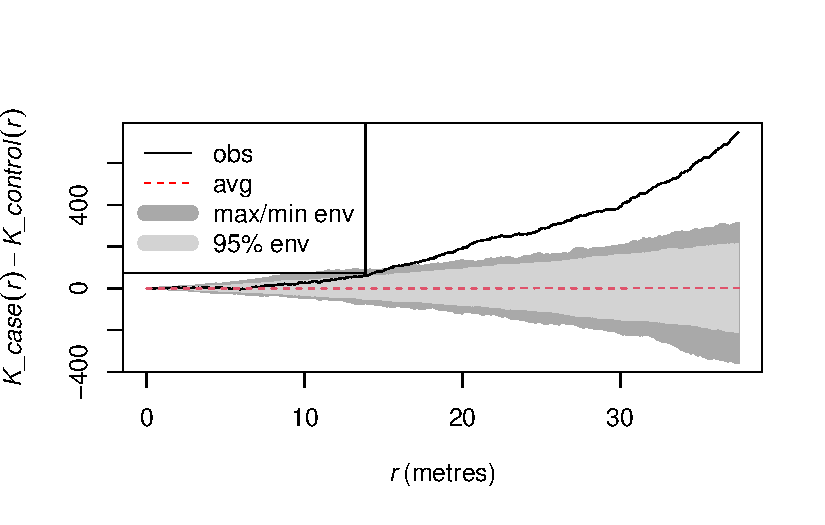
\includegraphics{cc-r-kd-hw_files/figure-pdf/unnamed-chunk-6-2.pdf}

}

\end{figure}

\begin{quote}
It appears that beyond around r=15 meters spatial scale, the oak trees
show evidence of clustering relative to the birch trees. To confirm, we
can look at the summary function for the kdest object.
\end{quote}

\begin{Shaded}
\begin{Highlighting}[]
\FunctionTok{summary}\NormalTok{(kdenv)}
\end{Highlighting}
\end{Shaded}

\begin{verbatim}
KD(r) > upper envelope limit for the following r:
0.7319336 
12.80884 
13.68716 to 13.76035 
14.05312 to 37.475 
\end{verbatim}

\begin{quote}
From the summary results we can see that there is evidence of clustering
of the oak trees relative to the controls for the spatial distance
ranges specified.
\end{quote}

\hypertarget{g.}{%
\subsection{g.}\label{g.}}

Perform a global test for clustering of the oak trees relative to the
birch trees using the \(KD_+\) statistic. Interpret the results.

\begin{Shaded}
\begin{Highlighting}[]
\FunctionTok{kdplus.test}\NormalTok{(kdenv)}
\end{Highlighting}
\end{Shaded}

\begin{verbatim}

Diggle and Chetwynd (1991) test for difference in K functions

KD(r) = K_case(r) - K_control(r)
case label:  oak 
control label:  birch 

null hypothesis: KD(r) = 0 for all r between 0 and 37.475 
alternative hypothesis: KD(r) > 0 for at least one r between 0 and 37.475 
test statistic: 1655.556 
p-value: 0.002 
nsim: 499 
simulation procedure: random labeling
\end{verbatim}

\begin{quote}
The global test p-value allows us to conclude that there is evidence of
clustering in the cases relative to the controls for at least 1 value of
r between 0 and 37.475. This outcome is in line with our plot showing
the 95\% confidence bands.
\end{quote}

\hypertarget{problem-2}{%
\section{Problem 2}\label{problem-2}}

The \texttt{paracou} data set in the \textbf{spatstat} package contains
data for Kimboto trees observed in Paracou, French Guiana. Let the
juveniles be the controls and adults be the cases. Use a bandwidth of 40
when estimating the densities of the juveniles and 65 for the adults.
Use a bandwidth of 52.5 when estimating the log ratio of spatial
densities.

\hypertarget{a.-1}{%
\subsection{a.}\label{a.-1}}

Create a plot of the of the point pattern that distinguishes between the
two types of trees. Do you notice any evidence of clusters? Explain.

\begin{Shaded}
\begin{Highlighting}[]
\NormalTok{kimboto }\OtherTok{\textless{}{-}}\NormalTok{ spatstat.data}\SpecialCharTok{::}\NormalTok{paracou}

\FunctionTok{plot}\NormalTok{(kimboto,}\AttributeTok{cols=}\FunctionTok{c}\NormalTok{(}\StringTok{\textquotesingle{}blue\textquotesingle{}}\NormalTok{,}\StringTok{\textquotesingle{}green\textquotesingle{}}\NormalTok{),}\AttributeTok{main =} \StringTok{\textquotesingle{}Kimboto Juvenile and Adult Locations\textquotesingle{}}\NormalTok{)}
\end{Highlighting}
\end{Shaded}

\begin{figure}[H]

{\centering 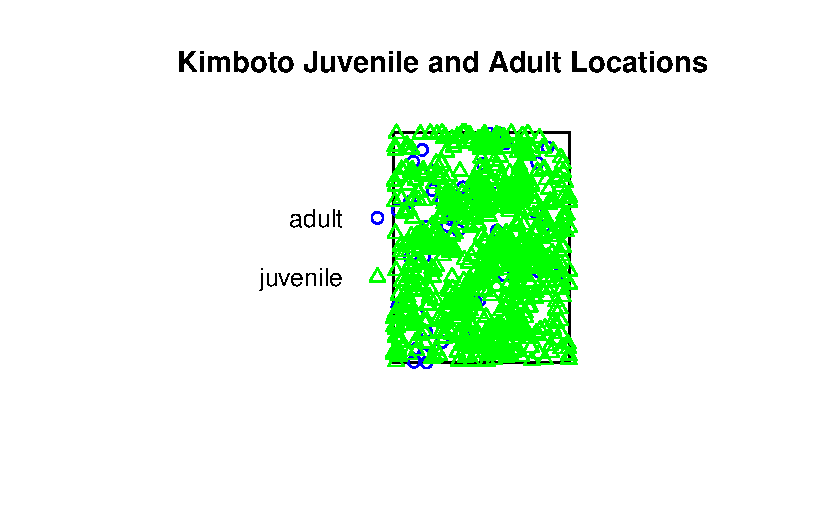
\includegraphics{cc-r-kd-hw_files/figure-pdf/unnamed-chunk-9-1.pdf}

}

\end{figure}

\begin{quote}
At a glance, there appears to be significantly more clustering in the
juvenile kimboto locations relative to the adult locations.
\end{quote}

\hypertarget{b.-1}{%
\subsection{b.}\label{b.-1}}

Create contour plots of the spatial density function for the adult and
juvenile trees. Use a bandwidth of 65 for the adult trees and 40 for the
juvenile trees. Do any differences jump out to you?

\begin{Shaded}
\begin{Highlighting}[]
\NormalTok{adult }\OtherTok{\textless{}{-}} \FunctionTok{which}\NormalTok{(kimboto}\SpecialCharTok{$}\NormalTok{marks }\SpecialCharTok{==} \StringTok{\textquotesingle{}adult\textquotesingle{}}\NormalTok{)}
\NormalTok{juvenile }\OtherTok{\textless{}{-}} \FunctionTok{which}\NormalTok{(kimboto}\SpecialCharTok{$}\NormalTok{marks }\SpecialCharTok{==} \StringTok{\textquotesingle{}juvenile\textquotesingle{}}\NormalTok{)}



\NormalTok{adult\_sp }\OtherTok{\textless{}{-}} \FunctionTok{spdensity}\NormalTok{(kimboto[adult],}\AttributeTok{sigma=}\DecValTok{65}\NormalTok{)}
\NormalTok{juv\_sp }\OtherTok{\textless{}{-}} \FunctionTok{spdensity}\NormalTok{(kimboto[juvenile],}\AttributeTok{sigma=}\DecValTok{40}\NormalTok{)}



\CommentTok{\# contour plot of adult kimbotos with title}
\FunctionTok{contour}\NormalTok{(adult\_sp, }\AttributeTok{nlevels =} \DecValTok{15}\NormalTok{, }\AttributeTok{main =} \StringTok{""}\NormalTok{)}
\FunctionTok{title}\NormalTok{(}\StringTok{"Adult, bandwidth = 65"}\NormalTok{)}
\end{Highlighting}
\end{Shaded}

\begin{figure}[H]

{\centering 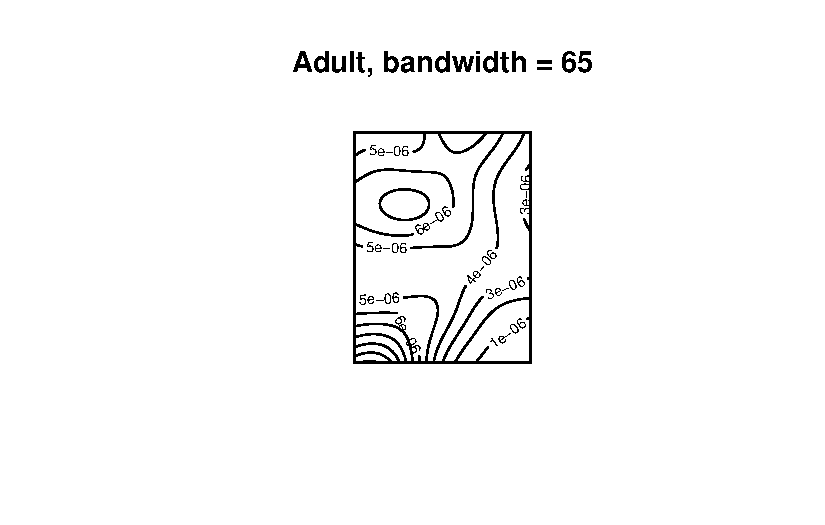
\includegraphics{cc-r-kd-hw_files/figure-pdf/unnamed-chunk-10-1.pdf}

}

\end{figure}

\begin{Shaded}
\begin{Highlighting}[]
\CommentTok{\# contour plot of juveniles, with title}
\FunctionTok{contour}\NormalTok{(juv\_sp, }\AttributeTok{nlevels =} \DecValTok{15}\NormalTok{, }\AttributeTok{main =} \StringTok{""}\NormalTok{)}
\FunctionTok{title}\NormalTok{(}\StringTok{"Juvenile, bandwidth = 40"}\NormalTok{)}
\end{Highlighting}
\end{Shaded}

\begin{figure}[H]

{\centering 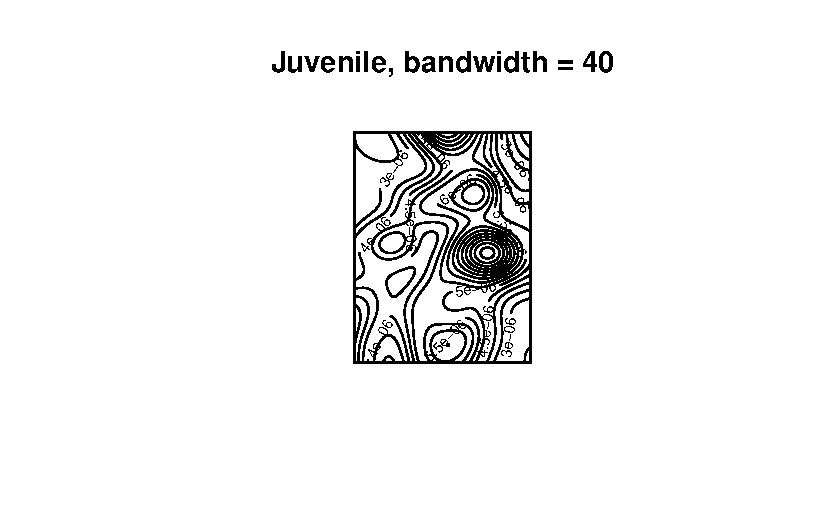
\includegraphics{cc-r-kd-hw_files/figure-pdf/unnamed-chunk-10-2.pdf}

}

\end{figure}

\begin{quote}
The Juvenile Kimboto relative intensities appear to vary much more than
the adult kimbotos and do not seem to match up to the adult contours.
\end{quote}

\hypertarget{c.-1}{%
\subsection{c.}\label{c.-1}}

Estimate the log ratio of the spatial density of the adult trees
relative to the juvenile trees (\(r(s)\)) using a bandwidth of 52.5.
Create a contour plot of the log ratio. Which areas are most
inconsistent with the belief that the spatial densities for the two
types of trees are the same?

\begin{Shaded}
\begin{Highlighting}[]
\CommentTok{\# log ratio of spatial densities}
\NormalTok{r\_adult }\OtherTok{=} \FunctionTok{logrr}\NormalTok{(kimboto, }\AttributeTok{case =} \StringTok{"adult"}\NormalTok{, }\AttributeTok{sigma =} \FloatTok{52.5}\NormalTok{)}
\end{Highlighting}
\end{Shaded}

\begin{verbatim}
adult has been selected as the case group
\end{verbatim}

\begin{Shaded}
\begin{Highlighting}[]
\CommentTok{\# contour plot of r\_adult}
\FunctionTok{contour}\NormalTok{(r\_adult, }\AttributeTok{lty =} \FunctionTok{c}\NormalTok{(}\DecValTok{1}\NormalTok{, }\DecValTok{1}\NormalTok{, }\DecValTok{1}\NormalTok{, }\DecValTok{1}\NormalTok{, }\DecValTok{2}\NormalTok{, }\DecValTok{1}\NormalTok{),}
        \AttributeTok{lwd =} \FunctionTok{c}\NormalTok{(}\DecValTok{1}\NormalTok{, }\DecValTok{1}\NormalTok{, }\DecValTok{1}\NormalTok{, }\DecValTok{1}\NormalTok{, }\DecValTok{1}\NormalTok{, }\DecValTok{2}\NormalTok{), }\AttributeTok{main =} \StringTok{""}\NormalTok{)}
\FunctionTok{title}\NormalTok{(}\StringTok{"Gaussian kernel, Bandwidth = 52.5"}\NormalTok{)}
\end{Highlighting}
\end{Shaded}

\begin{figure}[H]

{\centering 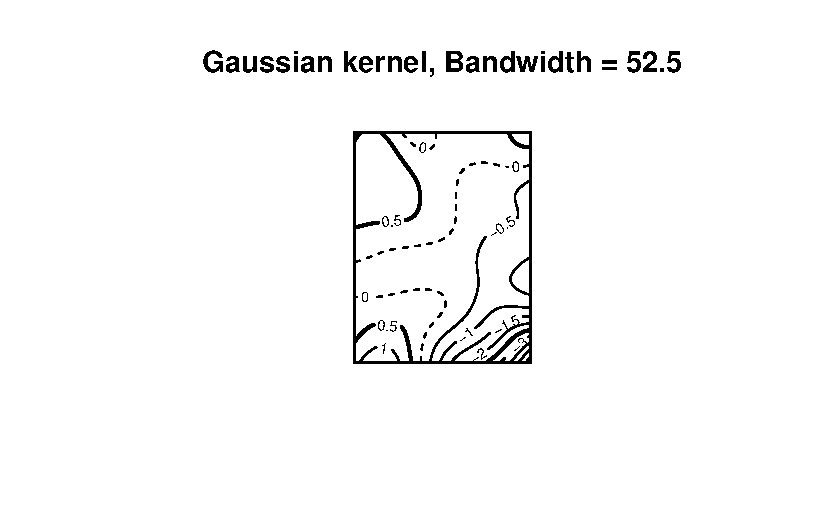
\includegraphics{cc-r-kd-hw_files/figure-pdf/unnamed-chunk-11-1.pdf}

}

\end{figure}

\begin{quote}
The region least consistent with the belief that the two types of trees
have the same spatial densities are in the bottom right and bottom left
of the plot.
\end{quote}

\hypertarget{d.-1}{%
\subsection{d.}\label{d.-1}}

Construct pointwise 95\% tolerance envelopes for \(r(s)\) using 499 data
sets simulated under the random labeling hypothesis. Plot the regions
above and below the tolerance envelopes in different colors. Overlay the
contour plot of \(\tilde{r}(s)\)). What can you conclude?

\begin{Shaded}
\begin{Highlighting}[]
\CommentTok{\# construct 95\% tolerance envelopes for log relative risk}
\NormalTok{lrr\_adult }\OtherTok{=} \FunctionTok{logrr}\NormalTok{(kimboto, }\AttributeTok{sigma =} \FloatTok{52.5}\NormalTok{, }\AttributeTok{case =} \StringTok{\textquotesingle{}adult\textquotesingle{}}\NormalTok{, }\AttributeTok{nsim =} \DecValTok{499}\NormalTok{,}
                \AttributeTok{level =} \FloatTok{0.95}\NormalTok{)}
\end{Highlighting}
\end{Shaded}

\begin{verbatim}
adult has been selected as the case group
\end{verbatim}

\begin{Shaded}
\begin{Highlighting}[]
\FunctionTok{plot}\NormalTok{(lrr\_adult)}
\end{Highlighting}
\end{Shaded}

\begin{figure}[H]

{\centering 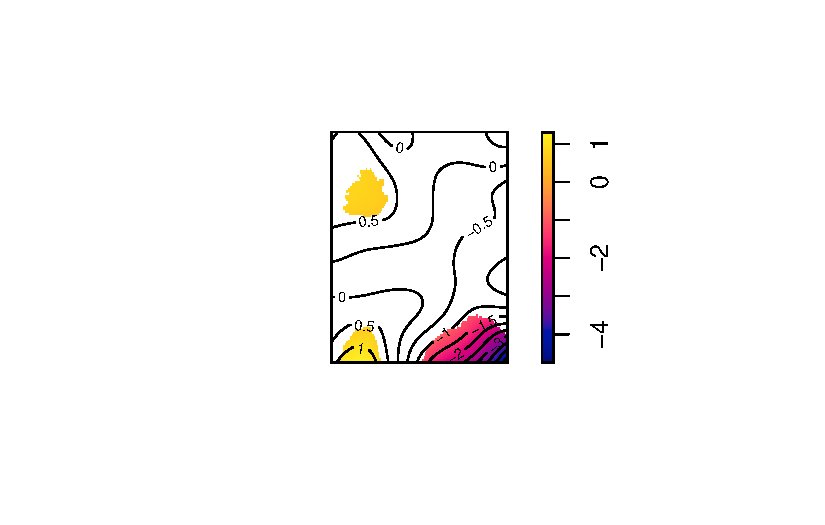
\includegraphics{cc-r-kd-hw_files/figure-pdf/unnamed-chunk-12-1.pdf}

}

\end{figure}

\begin{quote}
From the overlaid spatial densities we can see evidence of the control
juvenile trees clustering relative to the case `adult' trees in the
bottom right area, whereas in the top and bottom left areas marked in
yellow we see evidence of clustering for the case `adult' trees relative
to the control `juvenile' trees.
\end{quote}

\hypertarget{e.-1}{%
\subsection{e.}\label{e.-1}}

Perform a global test of clustering using \(\tilde{r}(s)\)). Is there
convincing evidence of clustering of one group relative to the other for
at least one location in the study area?.

\begin{Shaded}
\begin{Highlighting}[]
\FunctionTok{logrr.test}\NormalTok{(lrr\_adult)}
\end{Highlighting}
\end{Shaded}

\begin{verbatim}

Kelsall and Diggle (1995) test for log relative risk

r(s) = ln[f(s)/g(s)]
f(s) = spatial density of cases at location s
g(s) = spatial density of controls at location s
case label:  adult 
control label:  juvenile 

null hypothesis: r(s) = 0 for all s in study area
alternative hypothesis: r(s) != 0 for at least one s in study area
test statistic: 125222.1 
p-value: 0.056 
nsim: 499 
simulation procedure: random labeling
\end{verbatim}

\begin{quote}
At the alpha=.05 level, we can reject the null hypthesis that the
spatial densities of the two types of trees are the same. This is in
line our observed spatial density overlaid contour plot.
\end{quote}

\hypertarget{f.-1}{%
\subsection{f.}\label{f.-1}}

Construct a plot for the difference in K functions between the adult
trees and the juvenile trees. Also include min/max envelopes for this
difference using 499 simulated data sets under the random labeling
hypothesis. Also construct 95\% pointwise tolerance envelopes. Also
include the mean difference from the simulations. Provide a legend
labeling these things. Are there any spatial scales for which the adult
trees are more clustered than the juvenile trees in comparison to what
we expect under the random labeling hypothesis (or vice versa)? If so,
what scales?

\begin{Shaded}
\begin{Highlighting}[]
\DocumentationTok{\#\#\# difference in K functions}
\CommentTok{\# estimate K function for adult and juvenile,}
\CommentTok{\# take their difference}
\NormalTok{kd }\OtherTok{=} \FunctionTok{kdest}\NormalTok{(kimboto, }\AttributeTok{case =} \StringTok{\textquotesingle{}adult\textquotesingle{}}\NormalTok{)}
\end{Highlighting}
\end{Shaded}

\begin{verbatim}
adult has been selected as the case group
\end{verbatim}

\begin{Shaded}
\begin{Highlighting}[]
\CommentTok{\# plot estimated and theoretical KD (under RLH)}
\FunctionTok{plot}\NormalTok{(kd, }\FunctionTok{cbind}\NormalTok{(iso, theo) }\SpecialCharTok{\textasciitilde{}}\NormalTok{ r, }\AttributeTok{legend =} \ConstantTok{TRUE}\NormalTok{, }\AttributeTok{main =} \StringTok{""}\NormalTok{)}
\end{Highlighting}
\end{Shaded}

\begin{figure}[H]

{\centering 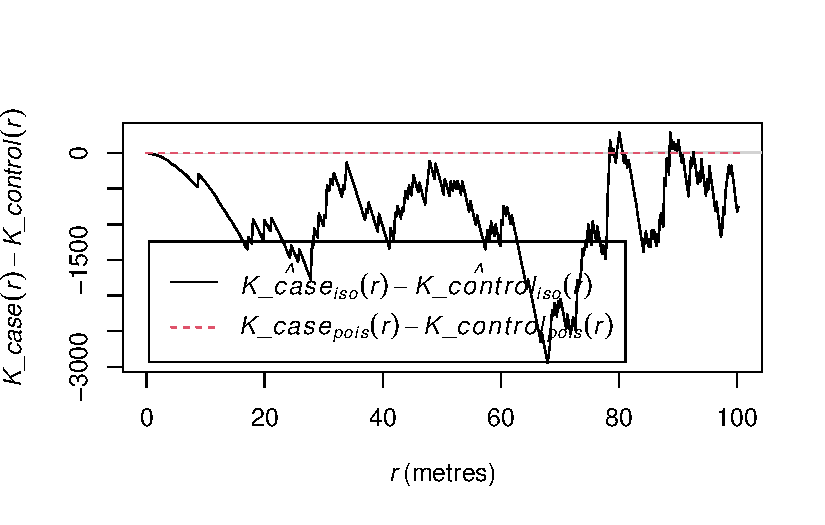
\includegraphics{cc-r-kd-hw_files/figure-pdf/unnamed-chunk-14-1.pdf}

}

\end{figure}

\begin{Shaded}
\begin{Highlighting}[]
\CommentTok{\# construct envelopes using 499 randomly labeled data sets}

\NormalTok{kdenv }\OtherTok{=} \FunctionTok{kdest}\NormalTok{(kimboto, }\AttributeTok{case =} \StringTok{"adult"}\NormalTok{, }\AttributeTok{nsim =} \DecValTok{499}\NormalTok{,}
              \AttributeTok{level =} \FloatTok{0.95}\NormalTok{)}
\end{Highlighting}
\end{Shaded}

\begin{verbatim}
adult has been selected as the case group
\end{verbatim}

\begin{verbatim}
Generating 499 simulations by evaluating expression  ...
1, 2, 3, .5....10....15....20....25....30....35....40....45....50..
..55....60....65....70....75....80....85....90....95....100....105....110
....115....120....125....130....135....140....145....150....155....160....165...
.170....175....180....185....190....195....200....205....210....215....220....225.
...230....235....240....245....250....255....260....265....270....275....280....
285....290....295....300....305....310....315....320....325....330....335....340..
..345....350....355....360....365....370....375....380....385....390....395....400
....405....410....415....420....425....430....435....440....445....450....455...
.460....465....470....475....480....485....490....495...
499.

Done.
\end{verbatim}

\begin{Shaded}
\begin{Highlighting}[]
\FunctionTok{plot}\NormalTok{(kdenv,}\AttributeTok{ylab=}\StringTok{\textquotesingle{}K Difference\textquotesingle{}}\NormalTok{)}
\FunctionTok{legend}\NormalTok{(}\StringTok{"topleft"}\NormalTok{, }\AttributeTok{legend =} \FunctionTok{c}\NormalTok{(}\StringTok{"obs"}\NormalTok{, }\StringTok{"avg"}\NormalTok{, }\StringTok{"max/min env"}\NormalTok{, }\StringTok{"95\% env"}\NormalTok{),}
       \AttributeTok{lty =} \FunctionTok{c}\NormalTok{(}\DecValTok{1}\NormalTok{, }\DecValTok{2}\NormalTok{, }\DecValTok{1}\NormalTok{, }\DecValTok{2}\NormalTok{), }\AttributeTok{col =} \FunctionTok{c}\NormalTok{(}\StringTok{"black"}\NormalTok{, }\StringTok{"red"}\NormalTok{, }\StringTok{"darkgrey"}\NormalTok{, }\StringTok{"lightgrey"}\NormalTok{),}
       \AttributeTok{lwd =} \FunctionTok{c}\NormalTok{(}\DecValTok{1}\NormalTok{, }\DecValTok{1}\NormalTok{, }\DecValTok{10}\NormalTok{, }\DecValTok{10}\NormalTok{))}
\end{Highlighting}
\end{Shaded}

\begin{figure}[H]

{\centering 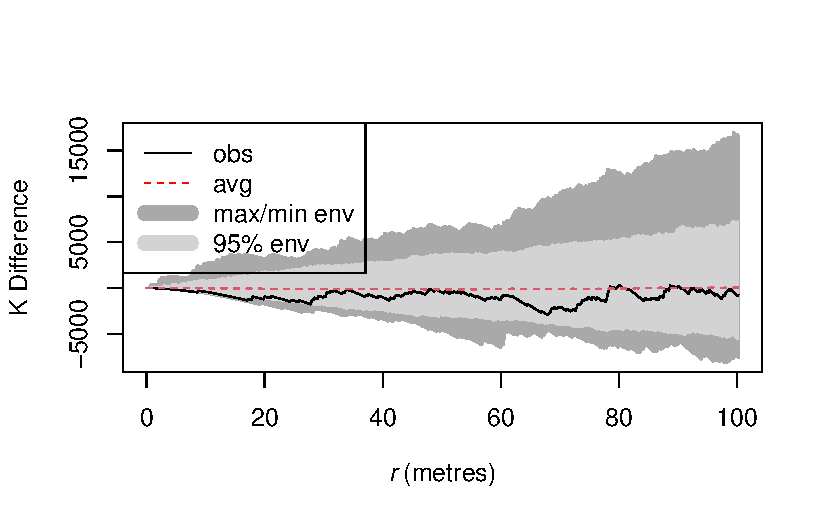
\includegraphics{cc-r-kd-hw_files/figure-pdf/unnamed-chunk-14-2.pdf}

}

\end{figure}

\begin{quote}
It appears that for many spatial densities between 0 and 25 we see
evidence of clustering of the control juvenile trees relative to the
adult case trees. To confirm which values exactly, we can use the
summary function for the kdest object.
\end{quote}

\begin{Shaded}
\begin{Highlighting}[]
\FunctionTok{summary}\NormalTok{(kdenv)}
\end{Highlighting}
\end{Shaded}

\begin{verbatim}
KD(r) < lower envelope limit for the following r:
1.565847 to 8.612158 
12.91824 to 17.81151 
27.79378 
\end{verbatim}

\hypertarget{g.-1}{%
\subsection{g.}\label{g.-1}}

Perform a global test for clustering of the adult trees relative to the
juvenile trees using the \(KD_+\) statistic. Interpret the results.

\begin{Shaded}
\begin{Highlighting}[]
\FunctionTok{kdplus.test}\NormalTok{(kdenv)}
\end{Highlighting}
\end{Shaded}

\begin{verbatim}

Diggle and Chetwynd (1991) test for difference in K functions

KD(r) = K_case(r) - K_control(r)
case label:  adult 
control label:  juvenile 

null hypothesis: KD(r) = 0 for all r between 0 and 100.2142 
alternative hypothesis: KD(r) > 0 for at least one r between 0 and 100.2142 
test statistic: -362.6496 
p-value: 0.806 
nsim: 499 
simulation procedure: random labeling
\end{verbatim}

\begin{quote}
The high p-value does not allow us to reject the null hypothesis,
however since the alternative hypothesis is one sided for KD(r)
\textgreater{} 0 this test does not check for clustering of the controls
relative to the cases. Were we to swap the `case' and `control' labels
of the kimboto trees then we might expect to see a smaller p-value,
given the plot of the kdest object.
\end{quote}

\hypertarget{problem-3}{%
\section{Problem 3}\label{problem-3}}

Let \(\lambda_0(s)\) denote a control intensity function and
\(\lambda_1(s)\) denote a case intensity function defined over a study
area \(D\). Assume that \(\lambda_1(s)=c\lambda_0(s)\) for all
\(s\in D\). Show that in this case, \(r(s)=0\) for all \(s\in D\).

\hypertarget{problem-4}{%
\section{Problem 4}\label{problem-4}}

Let \(\lambda_0(s)\) denote a control intensity function and
\(\lambda_1(s)\) denote a case intensity function defined over a study
area \(D\). Assume that \(\lambda_1(s)=c\lambda_0(s)\) for all
\(s\in D\).. Show that \(f(s)=g(s)\) for all \(s\in D\), where \(f\) and
\(g\) are the spatial densities of the cases and controls, respectively.



\end{document}
